\chapter{Tomando decis\~oes}

Um c\'odigo pode ter rotinas para a resolu\c{c}\~ao de um determinado problema necessitem serem seguidos, enquanto outros n\~ao o sejam. 
Rotinas s\~ao sequ\^encias de linhas de c\'odigo. A cria\c{c}\~ao de uma estrutura de decis\~ao permite controlar quais rotinas devem ser executadas em 
detrimento de outras. Para este fim o Perl possui fun\c{c}\~oes de compara\c{c}\~ao (\textit{if, else} e \textit{elsif}). \textit{if} traduzido para o 
portugu\^es fica ''se''. Um exemplo de seu funcionamento \'e apresentado na figura 11.   

\begin{figure}[!htb]
	\centering
	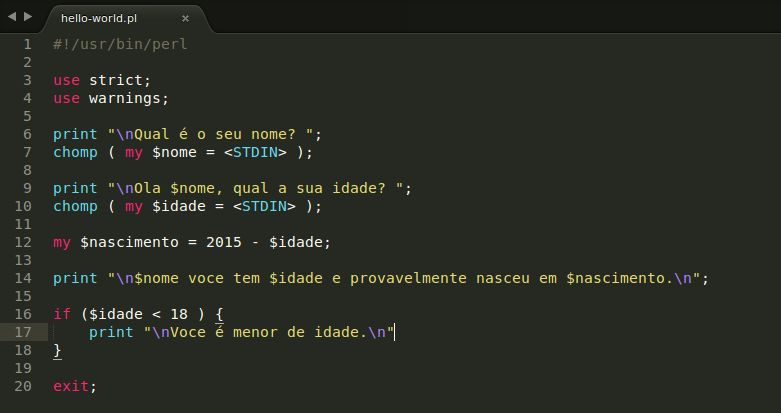
\includegraphics[width=0.7\textwidth]{../5_figuras/image11}
	\caption{Algoritmo com estrutura de decis\~ao}
\end{figure}

Na figura 11, linha 16 pode-se ver o que o \textit{if} compara se a vari\'avel que cont\'em a idade informada pelo usu\'ario \'e menor que 18, caso a idade 
seja menor, \'e requisitado que um trecho de c\'odigo respons\'avel por imprimir a mensagem ''Voc\^e \'e menor de idade'' para a sa\'ida padr\~ao seja chamada.

A sa\'ida \'e apresentada na figura 12.

\begin{figure}[!htb]
	\centering
	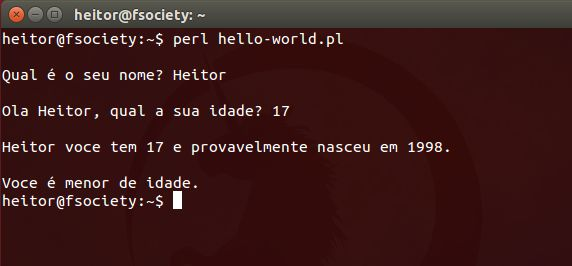
\includegraphics[width=0.7\textwidth]{../5_figuras/image12}
	\caption{Sa\'ida do algoritmo com estrutura de decis\~ao}
\end{figure}

Com o \textit{if} pode-se comparar tanto valores num\'ericos quanto cadeias de caracteres (\textit{strings}). O \textit{else} pode ser traduzido como 
''sen\~ao'', seu uso em conjunto com o if \'e caracteriza uma estrutura de decis\~ao composta, seu funcionamento pode ser visto na figura 13.

\begin{figure}[!htb]
	\centering
	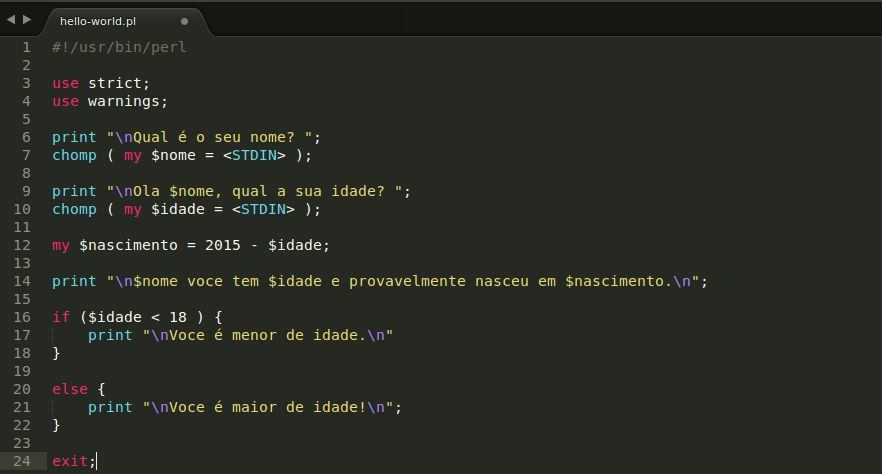
\includegraphics[width=0.7\textwidth]{../5_figuras/image13}
	\caption{Algoritmo com estrutura de decis\~ao composta}
\end{figure}

\clearpage 

Logicamente se a idade do usu\'ario n\~ao for menor que 18, ent\~ao ele ser\'a  maior de idade, como apresentado na figura 14.

\begin{figure}[!htb]
	\centering
	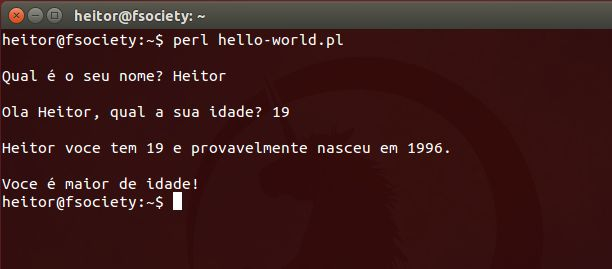
\includegraphics[width=0.5\textwidth]{../5_figuras/image14}
	\caption{Sa\'ida do algoritmo com estrutura de decis\~ao composta}
\end{figure}

E finalmente, o \textit{elsif}, sua tradu\c{c}\~ao \'e equivalente a ''sen\~ao se''. O uso conjuto de \textit{if}, \textit{elsif} e \textit{else} permite uma
estrutura de decis\~ao muito mais abrangente e precisa, chamada de estrutura de decis\~ao completa, como apresentado na figura 15.

\begin{figure}[!htb]
	\centering
	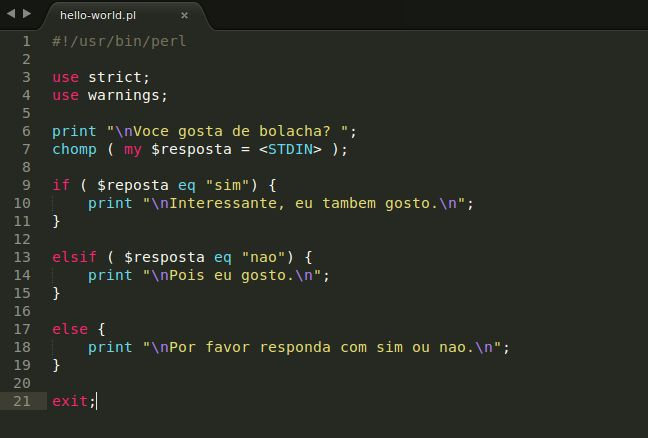
\includegraphics[width=0.6\textwidth]{../5_figuras/image15}
	\caption{Algoritmo com estrutura de decis\~ao completa}
\end{figure}

Na figura 16, linha 9 observa-se que a resposta dada foi  ''sim'', j\'a na linha 13 observa-se outro caso onde a resposta dada foi ''n\~ao'', caso 
a resposta dada n\~ao fosse igual a nenhum dos casos abordados nas condi\c{c}\~oes anteriores da estrutura de decis\~ao o \textit{else} pede para responder 
corretamente. 

\begin{figure}[!htb]
	\centering
	
\includegraphics[width=0.4\textwidth]{../5_figuras/image16}
	\caption{Sa\'ida do algoritmo com estrutura de decis\~ao completa}
\end{figure}




